\documentclass[10,portrait]{article}
\usepackage{lmodern}
\usepackage{amssymb,amsmath}
\usepackage{ifxetex,ifluatex}
\usepackage{fixltx2e} % provides \textsubscript
\ifnum 0\ifxetex 1\fi\ifluatex 1\fi=0 % if pdftex
  \usepackage[T1]{fontenc}
  \usepackage[utf8]{inputenc}
\else % if luatex or xelatex
  \ifxetex
    \usepackage{mathspec}
  \else
    \usepackage{fontspec}
  \fi
  \defaultfontfeatures{Ligatures=TeX,Scale=MatchLowercase}
\fi
% use upquote if available, for straight quotes in verbatim environments
\IfFileExists{upquote.sty}{\usepackage{upquote}}{}
% use microtype if available
\IfFileExists{microtype.sty}{%
\usepackage[]{microtype}
\UseMicrotypeSet[protrusion]{basicmath} % disable protrusion for tt fonts
}{}
\PassOptionsToPackage{hyphens}{url} % url is loaded by hyperref
\usepackage[unicode=true]{hyperref}
\PassOptionsToPackage{usenames,dvipsnames}{color} % color is loaded by hyperref
\hypersetup{
            pdftitle={Tic-Tac-Toe: Individual-based spatial consumer-resource disease transmission model for predicting parasite loading on nutrient cycling in ecosystems},
            colorlinks=true,
            linkcolor=pink,
            citecolor=red,
            urlcolor=blue,
            breaklinks=true}
\urlstyle{same}  % don't use monospace font for urls
\usepackage[margin=1in]{geometry}
\usepackage[]{biblatex}
\usepackage{color}
\usepackage{fancyvrb}
\newcommand{\VerbBar}{|}
\newcommand{\VERB}{\Verb[commandchars=\\\{\}]}
\DefineVerbatimEnvironment{Highlighting}{Verbatim}{commandchars=\\\{\}}
% Add ',fontsize=\small' for more characters per line
\usepackage{framed}
\definecolor{shadecolor}{RGB}{248,248,248}
\newenvironment{Shaded}{\begin{snugshade}}{\end{snugshade}}
\newcommand{\KeywordTok}[1]{\textcolor[rgb]{0.13,0.29,0.53}{\textbf{#1}}}
\newcommand{\DataTypeTok}[1]{\textcolor[rgb]{0.13,0.29,0.53}{#1}}
\newcommand{\DecValTok}[1]{\textcolor[rgb]{0.00,0.00,0.81}{#1}}
\newcommand{\BaseNTok}[1]{\textcolor[rgb]{0.00,0.00,0.81}{#1}}
\newcommand{\FloatTok}[1]{\textcolor[rgb]{0.00,0.00,0.81}{#1}}
\newcommand{\ConstantTok}[1]{\textcolor[rgb]{0.00,0.00,0.00}{#1}}
\newcommand{\CharTok}[1]{\textcolor[rgb]{0.31,0.60,0.02}{#1}}
\newcommand{\SpecialCharTok}[1]{\textcolor[rgb]{0.00,0.00,0.00}{#1}}
\newcommand{\StringTok}[1]{\textcolor[rgb]{0.31,0.60,0.02}{#1}}
\newcommand{\VerbatimStringTok}[1]{\textcolor[rgb]{0.31,0.60,0.02}{#1}}
\newcommand{\SpecialStringTok}[1]{\textcolor[rgb]{0.31,0.60,0.02}{#1}}
\newcommand{\ImportTok}[1]{#1}
\newcommand{\CommentTok}[1]{\textcolor[rgb]{0.56,0.35,0.01}{\textit{#1}}}
\newcommand{\DocumentationTok}[1]{\textcolor[rgb]{0.56,0.35,0.01}{\textbf{\textit{#1}}}}
\newcommand{\AnnotationTok}[1]{\textcolor[rgb]{0.56,0.35,0.01}{\textbf{\textit{#1}}}}
\newcommand{\CommentVarTok}[1]{\textcolor[rgb]{0.56,0.35,0.01}{\textbf{\textit{#1}}}}
\newcommand{\OtherTok}[1]{\textcolor[rgb]{0.56,0.35,0.01}{#1}}
\newcommand{\FunctionTok}[1]{\textcolor[rgb]{0.00,0.00,0.00}{#1}}
\newcommand{\VariableTok}[1]{\textcolor[rgb]{0.00,0.00,0.00}{#1}}
\newcommand{\ControlFlowTok}[1]{\textcolor[rgb]{0.13,0.29,0.53}{\textbf{#1}}}
\newcommand{\OperatorTok}[1]{\textcolor[rgb]{0.81,0.36,0.00}{\textbf{#1}}}
\newcommand{\BuiltInTok}[1]{#1}
\newcommand{\ExtensionTok}[1]{#1}
\newcommand{\PreprocessorTok}[1]{\textcolor[rgb]{0.56,0.35,0.01}{\textit{#1}}}
\newcommand{\AttributeTok}[1]{\textcolor[rgb]{0.77,0.63,0.00}{#1}}
\newcommand{\RegionMarkerTok}[1]{#1}
\newcommand{\InformationTok}[1]{\textcolor[rgb]{0.56,0.35,0.01}{\textbf{\textit{#1}}}}
\newcommand{\WarningTok}[1]{\textcolor[rgb]{0.56,0.35,0.01}{\textbf{\textit{#1}}}}
\newcommand{\AlertTok}[1]{\textcolor[rgb]{0.94,0.16,0.16}{#1}}
\newcommand{\ErrorTok}[1]{\textcolor[rgb]{0.64,0.00,0.00}{\textbf{#1}}}
\newcommand{\NormalTok}[1]{#1}
\usepackage{graphicx,grffile}
\makeatletter
\def\maxwidth{\ifdim\Gin@nat@width>\linewidth\linewidth\else\Gin@nat@width\fi}
\def\maxheight{\ifdim\Gin@nat@height>\textheight\textheight\else\Gin@nat@height\fi}
\makeatother
% Scale images if necessary, so that they will not overflow the page
% margins by default, and it is still possible to overwrite the defaults
% using explicit options in \includegraphics[width, height, ...]{}
\setkeys{Gin}{width=\maxwidth,height=\maxheight,keepaspectratio}
\IfFileExists{parskip.sty}{%
\usepackage{parskip}
}{% else
\setlength{\parindent}{0pt}
\setlength{\parskip}{6pt plus 2pt minus 1pt}
}
\setlength{\emergencystretch}{3em}  % prevent overfull lines
\providecommand{\tightlist}{%
  \setlength{\itemsep}{0pt}\setlength{\parskip}{0pt}}
\setcounter{secnumdepth}{0}
% Redefines (sub)paragraphs to behave more like sections
\ifx\paragraph\undefined\else
\let\oldparagraph\paragraph
\renewcommand{\paragraph}[1]{\oldparagraph{#1}\mbox{}}
\fi
\ifx\subparagraph\undefined\else
\let\oldsubparagraph\subparagraph
\renewcommand{\subparagraph}[1]{\oldsubparagraph{#1}\mbox{}}
\fi

% set default figure placement to htbp
\makeatletter
\def\fps@figure{htbp}
\makeatother


\title{Tic-Tac-Toe: Individual-based spatial consumer-resource disease
transmission model for predicting parasite loading on nutrient cycling
in ecosystems}
\author{Matt Malishev, Emory University, USA\\
J. Trevor Vannatta, Purdue University, USA\\
Amanda Koltz, Washington University in St.~Louis, USA\\
Rachel Penczkowski, Washington University in St.~Louis, USA\\
Sharon Deem, Institute for Conservation Medicine, St.~Louis Zoo, USA\\
Vanessa Ezenwa, University of Georgia, USA\\
Zoe Johnson, Mississippi State University, USA\\
Aimee Classen, University of Vermont, USA\\
Maris Brenn-White, St.~Louis Zoo, USA\\
David Civitello, Emory University, USA}
\date{}

\begin{document}
\maketitle

{
\hypersetup{linkcolor=black}
\setcounter{tocdepth}{4}
\tableofcontents
}
~

Date: 2019-01-25\\
\texttt{R} version: 3.5.0\\
*Corresponding author:
\href{mailto:matthew.malishev@gmail.com}{\nolinkurl{matthew.malishev@gmail.com}}\\
This document can be found at
\url{https://github.com/darwinanddavis/tictactoe}

\newpage  

\subsection{Overview}\label{overview}

Develop the consumer-resource disease transmission model of parasite
loading on nutrient cycling in ecosystems as a spatial individual-based
model.

To forecast how resource biomass uptake and release by infected and
non-infected host populations varies under a disease mosaic landscape
driven by feedback between modes and rates of disease transmission and
costs of parasite occurrence and nutrient deposit in space and time.

The model applies the
\href{https://github.com/darwinanddavis/LECWorkingGroup}{nutrient-plant-susceptible-infectious
(NPSI) model} in a spatial landscape of resources, host populations, and
disease vector populations.

\subsection{The rundown}\label{the-rundown}

The model explores the transmission probability of diseases among host
populations in a simulated patchwork landscape of resource and disease
patches. The two main entities are host individuals (agents) and
patches. Hosts are mobile units that move throughout the model landscape
using user-defined movement/patch occurrence rules and aim to consume
the resource patches that provide them with energy to fuel their
growth/death rates. Individuals belong to host populations that are
either susceptible to infection risk (S) or infected with a disease (I).

The probability of a susceptible host becoming infected is determined
via two pathways:

\begin{itemize}
\item
  Encounter food and/or ground patches in the landscape that contain
  parasites, such as diseased food or infected waste (faeces or
  carcasses of infected hosts).
\item
  Encounter infected hosts on a shared food and/or ground patch.
\end{itemize}

Infected hosts can transmit parasites to susceptible hosts. Infected
hosts cannot be infected further, but can shed their parasites, after
which they reset their infection probability and become susceptible
again.

Patches in the landscape are either ground, resources, or infected
patches (ground or resources). Resource patch growth rates depend on
nutrient supply in a patch. Bare ground patches can become resource
patches when their nutrient load is sufficient to grow resources.
Resource patches are consumed if 1) the patch is occupied by
individual/multiple hosts and 2) the host requires energy.

All rates of nutrient supply, resource growth, and host population
densities are determined by the state variable ODEs (defined below).

\subsection{From individual to
population}\label{from-individual-to-population}

The model can be as simple or as complex as we want it to be. The best
way to build the model is to keep our main research questions at the
forefront as we modify the model assumptions. This will help us confine
the aims of the model and what we feed into it, which is limited by
available data.

The model uses individual hosts as units and patches as cells that
contain information on how the individual will update its current state
at each time step. For example, a host that begins the simulation at
time step 0 as susceptible will encounter food patches at different time
steps, which update its energetic state. If this host then encounters an
infected host at time step 5, the state of this newly infected host will
change to infected. This newly infected host then updates its current
energetic state at time step 6 to reflect the consequences of its body
condition being infected.

The nutrient and resource load of patches also varies per time step as
patches are updated with new nutrients, consumed by hosts, or infected
by infected products or carcasses.

While the units are the individual hosts, the patterns emerging from the
simulation are at the host population level. This keeps the transmission
dynamics within a susceptible/infected population framework that
corresponds to the output of biomass back into the landscape. The rates
of transmission and resource growth are at faster time scales than host
birth/death rates. Therefore, varying these rates and the values that
feed these rates will determine what the model simulations produce
throughout the different time and space scales.

\subsection{Methods}\label{methods}

\subsubsection{Model description}\label{model-description}

\textbf{State variables (units = biomass)}\\
N = nutrients in the landscape (biomass)\\
P = food in the landscape (plant biomass)\\
S = susceptible ungulate host population\\
I = infected ungulate host population

\textbf{Parameters}\\
r = intrinsic growth rate of plants\\
K = carrying capacity of plants\\
a = rate of nutrient addition\\
l = nutrient loss rate\\
fp = rate of plant nutrient uptake\\
\(\beta\) = transmission rate\\
es = assimilation efficiency of susceptible hosts\\
ei = assimilation efficiency of infected hosts\\
fs = feeding rate of susceptible hosts\\
fi = feeding rate of infected hosts\\
d = background host death rate\\
v = mortality rate from infection\\
ws = rate of waste production from susceptible hosts\\
wi = rate of waste production from infected hosts

\subsubsection{State variable ODEs}\label{state-variable-odes}

Nutrient growth (biomass)\\
\[
\frac
{dN}
{dt} = 
a - lN - fpNP + (d+ws)S + (d+v+wi)I  
\]

Food growth (biomass)\\
\[
\frac
{dP}
{dt} = 
fpNrP(1-(P/K)) - P(fsS+fiI) 
\]

Susceptible host density\\
\[
\frac
{dS}
{dt}
= P(esfsS + eifiI) - \beta S - (d+ws)S 
\]

Infected host density\\
\[
\frac
{dI}
{dt}
= \beta S - (d+v+wi)I 
\]

\begin{figure}
\centering
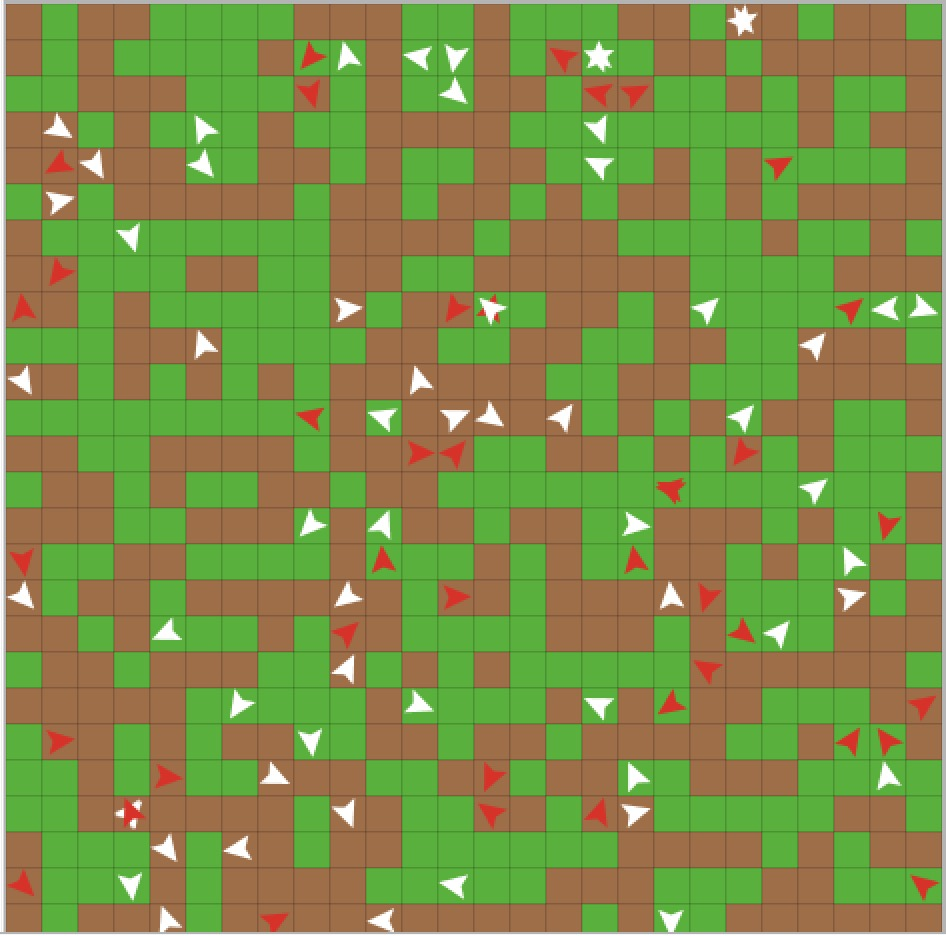
\includegraphics{landscape2.jpeg}
\caption{Example of what the model landscape might look like with food
patches (green), infected patches (brown), and host individuals (white =
S, red = I).}
\end{figure}

The interplay between the fast (e.g.~feeding, disease transmission) and
slow (e.g.~nutrient cycling, birth/death) rate dynamics at different
time and space scales generates emergent patterns for the different
state variable and parameter values we use to define the model starting
conditions and inputs.

\subsection{Questions to answer}\label{questions-to-answer}

Some examples of questions we could answer:

\begin{itemize}
\item
  What density of infected patches in the landscape increases
  transmission and mortality rates?
\item
  How does host density per patch drive disease transmission rates?
\item
  What density of infected resources drives direct mortality (host
  density per infected patch) versus indirect mortality (horizontal
  disease transmission from newly born infected hosts)?
\item
  How does persistence of infected host density shape infected patch
  arrangement in the landscape and ultimately exposure risk to
  susceptible hosts?
\item
  What density of infected hosts suppresses nutrient stocks to levels
  below unsustainable food growth?
\item
  Etc
\end{itemize}

\subsection{Extensions of the model}\label{extensions-of-the-model}

The model landscape can also include free-ranging, mobile disease
vectors, i.e.~mosquitoes and ticks, that have their own basic movement
rules. This can follow three modes:

\begin{itemize}
\item
  Opportunistic, where vectors follow correlated random walk in the
  landscape and host-vector encounter rates are probabilistic based on
  vector and susceptible host density per patch.
\item
  Recurring, where vector density in the landscape peaks according to
  regular rollout events throughout the simulation. This aims to follow
  vector occurrence patterns that correlate with predictable natural
  phenomena i.e.~seasonal fluctuations in humidity.
\item
  Episodic, where the landscape is `flooded' with vectors at given times
  throughout the simulation. This aims to replicate sudden disease
  outbreaks in a given spatial area that may correspond to climate,
  human-induced, and/or epidemic events.
\end{itemize}

\subsection{Appendix}\label{appendix}

Model code (from
\href{https://github.com/darwinanddavis/LECWorkingGroup}{nutrient-plant-susceptible-infectious
(NPSI) model})

\begin{Shaded}
\begin{Highlighting}[]
\NormalTok{##########################################################################################}
\NormalTok{################################# User inputs for model ##################################}
\NormalTok{##########################################################################################}

\CommentTok{# set your working directory }
\CommentTok{# E.g "/Users/malishev/dope_models/my_dope_model/"}
\NormalTok{wd <-}\StringTok{ "paste the path to where you saved the model here (with these quotes)"}
\KeywordTok{setwd}\NormalTok{(wd)}

\CommentTok{# set parameter ranges (min 0, max 1)}
\NormalTok{beta_access <-}\StringTok{ }\FloatTok{0.1} \CommentTok{# choose your beta value you want to plot at the end}
\NormalTok{death_access <-}\StringTok{ }\FloatTok{0.9} \CommentTok{# choose your death value you want to plot at the end}
\NormalTok{colvv <-}\StringTok{ "orange"} \CommentTok{# choose your plot line colour}

\NormalTok{## initial conditions}
\NormalTok{N <-}\StringTok{ }\DecValTok{200} \CommentTok{# size of nutrient biomass in env }
\NormalTok{P <-}\StringTok{ }\DecValTok{200} \CommentTok{# initial products in env}
\NormalTok{S <-}\StringTok{ }\DecValTok{20} \CommentTok{# num of susceptible hosts}
\NormalTok{In <-}\StringTok{ }\DecValTok{2} \CommentTok{# num of infected hosts }
\NormalTok{years <-}\StringTok{ }\DecValTok{100} \CommentTok{# number of years to run simulation}
\NormalTok{time.out <-}\StringTok{ }\FloatTok{0.01} \CommentTok{# simulation time step (0.01 = 1 year if years = 100) }
\end{Highlighting}
\end{Shaded}

\begin{Shaded}
\begin{Highlighting}[]
\NormalTok{##########################################################################################}
\NormalTok{##################################### Setup simulation model #############################}
\NormalTok{##########################################################################################}
\CommentTok{# set param space}
\NormalTok{beta_pars <-}\StringTok{ }\KeywordTok{seq}\NormalTok{(}\FloatTok{0.1}\NormalTok{,}\DecValTok{1}\NormalTok{,}\FloatTok{0.1}\NormalTok{) }\CommentTok{# transmission rate in model }
\NormalTok{death_pars <-}\StringTok{ }\KeywordTok{seq}\NormalTok{(}\FloatTok{0.1}\NormalTok{,}\DecValTok{1}\NormalTok{,}\FloatTok{0.1}\NormalTok{) }\CommentTok{# death rate in model}

\CommentTok{# desired outputs}
\NormalTok{out <-}\StringTok{ }\KeywordTok{list}\NormalTok{()}
\NormalTok{out_master <-}\StringTok{ }\KeywordTok{list}\NormalTok{() }\CommentTok{# NPSI output }
\NormalTok{out_tibble <-}\StringTok{ }\KeywordTok{tibble}\NormalTok{()}
\NormalTok{outplot <-}\StringTok{ }\KeywordTok{list}\NormalTok{()}
\NormalTok{param_space <-}\StringTok{ }\KeywordTok{list}\NormalTok{(beta_pars,death_pars) }\CommentTok{# summed parameter space }

\CommentTok{# create empty list}
\NormalTok{out_master <-}\StringTok{ }\KeywordTok{rep}\NormalTok{(}
  \KeywordTok{list}\NormalTok{(}\KeywordTok{structure}\NormalTok{(}\KeywordTok{list}\NormalTok{(}
    \DataTypeTok{pars =} \KeywordTok{numeric}\NormalTok{(), }
    \DataTypeTok{outs =} \KeywordTok{list}\NormalTok{()}
\NormalTok{    ),}
    \DataTypeTok{.Names =} \KeywordTok{c}\NormalTok{(}\StringTok{"Parameter"}\NormalTok{, }\StringTok{"Output"}\NormalTok{)))}
\NormalTok{    ,}\KeywordTok{prod}\NormalTok{(}\KeywordTok{as.numeric}\NormalTok{(}\KeywordTok{summary}\NormalTok{(param_space)[,}\DecValTok{1}\NormalTok{]))}
\NormalTok{  )}
\NormalTok{sc <-}\StringTok{ }\DecValTok{1} \CommentTok{# timer in simulation model }

\NormalTok{#############################################################################}
\CommentTok{# create simulation model  #############################}

\CommentTok{# to set pars as individual beta and death values}
\NormalTok{npsi_func <-}\StringTok{ }\ControlFlowTok{function}\NormalTok{()\{ }\CommentTok{# start npsi_func}
  
  \CommentTok{# ------- start simulation # ------- }
  \ControlFlowTok{for}\NormalTok{(beta }\ControlFlowTok{in}\NormalTok{ beta_pars)\{ }\CommentTok{# pass through beta values}
    \ControlFlowTok{for}\NormalTok{(death }\ControlFlowTok{in}\NormalTok{ death_pars)\{ }\CommentTok{# pass through death values }
\NormalTok{      parameters<-}\KeywordTok{c}\NormalTok{(}\DataTypeTok{r=}\FloatTok{0.2}\NormalTok{, }\DataTypeTok{K=}\DecValTok{100}\NormalTok{, }\DataTypeTok{a=}\DecValTok{500}\NormalTok{, }\DataTypeTok{l=}\DecValTok{5}\NormalTok{, }\DataTypeTok{fp=}\FloatTok{0.5}\NormalTok{, }\DataTypeTok{beta=}\NormalTok{beta, }
                    \DataTypeTok{es=}\FloatTok{0.1}\NormalTok{, }\DataTypeTok{ei=}\FloatTok{0.05}\NormalTok{, }\DataTypeTok{fs=}\FloatTok{0.2}\NormalTok{, }\DataTypeTok{fi=}\FloatTok{0.1}\NormalTok{,}
                    \DataTypeTok{d=}\NormalTok{death, }\DataTypeTok{v=}\FloatTok{0.1}\NormalTok{, }\DataTypeTok{ws=}\FloatTok{0.05}\NormalTok{, }\DataTypeTok{wi=}\FloatTok{0.09}\NormalTok{)}
      
\NormalTok{      state<-}\KeywordTok{c}\NormalTok{(}\DataTypeTok{N=}\NormalTok{N, }\DataTypeTok{P=}\NormalTok{P, }\DataTypeTok{S=}\NormalTok{S, }\DataTypeTok{I=}\NormalTok{In) }\CommentTok{# set initial conditions}
      
\NormalTok{      NPSI<-}\ControlFlowTok{function}\NormalTok{(t, state, parameters) \{ }
        \KeywordTok{with}\NormalTok{(}\KeywordTok{as.list}\NormalTok{(}\KeywordTok{c}\NormalTok{(state, parameters)),\{}
          
\NormalTok{          dN.dt <-}\StringTok{ }\NormalTok{a }\OperatorTok{-}\StringTok{ }\NormalTok{l}\OperatorTok{*}\NormalTok{N }\OperatorTok{-}\StringTok{ }\NormalTok{fp}\OperatorTok{*}\NormalTok{N}\OperatorTok{*}\NormalTok{P }\OperatorTok{+}\StringTok{ }\NormalTok{(d}\OperatorTok{+}\NormalTok{ws)}\OperatorTok{*}\NormalTok{S }\OperatorTok{+}\StringTok{ }\NormalTok{(d}\OperatorTok{+}\NormalTok{v}\OperatorTok{+}\NormalTok{wi)}\OperatorTok{*}\NormalTok{I  }\CommentTok{# nutrients in env}
\NormalTok{          dP.dt <-}\StringTok{ }\NormalTok{fp}\OperatorTok{*}\NormalTok{N}\OperatorTok{*}\NormalTok{r}\OperatorTok{*}\NormalTok{P}\OperatorTok{*}\NormalTok{(}\DecValTok{1}\OperatorTok{-}\NormalTok{(P}\OperatorTok{/}\NormalTok{K)) }\OperatorTok{-}\StringTok{ }\NormalTok{P}\OperatorTok{*}\NormalTok{(fs}\OperatorTok{*}\NormalTok{S}\OperatorTok{*+}\NormalTok{fi}\OperatorTok{*}\NormalTok{I) }\CommentTok{# plants produced  }
\NormalTok{          dS.dt <-}\StringTok{ }\NormalTok{P}\OperatorTok{*}\NormalTok{(es}\OperatorTok{*}\NormalTok{fs}\OperatorTok{*}\NormalTok{S }\OperatorTok{+}\StringTok{ }\NormalTok{ei}\OperatorTok{*}\NormalTok{fi}\OperatorTok{*}\NormalTok{I) }\OperatorTok{-}\StringTok{ }\NormalTok{beta}\OperatorTok{*}\NormalTok{S }\OperatorTok{-}\StringTok{ }\NormalTok{(d}\OperatorTok{+}\NormalTok{ws)}\OperatorTok{*}\NormalTok{S }\CommentTok{# susceptible hosts }
\NormalTok{          dI.dt <-}\StringTok{ }\NormalTok{beta}\OperatorTok{*}\NormalTok{S }\OperatorTok{-}\StringTok{ }\NormalTok{(d}\OperatorTok{+}\NormalTok{v}\OperatorTok{+}\NormalTok{wi)}\OperatorTok{*}\NormalTok{I }\CommentTok{# infected hosts }
          
          \KeywordTok{list}\NormalTok{(}\KeywordTok{c}\NormalTok{(dN.dt, dP.dt, dS.dt, dI.dt)) }\CommentTok{# compile outputs }
\NormalTok{        \})}
\NormalTok{      \} }\CommentTok{# end npsi function}
      
      \CommentTok{# -------  global output # ------- }
\NormalTok{      times <-}\StringTok{ }\KeywordTok{seq}\NormalTok{(}\DecValTok{0}\NormalTok{, years, }\DataTypeTok{by=}\NormalTok{time.out) }\CommentTok{# set time horizon for simulation (years)}
\NormalTok{      out <-}\StringTok{ }\KeywordTok{ode}\NormalTok{(}\DataTypeTok{y=}\NormalTok{state, }\DataTypeTok{times=}\NormalTok{times, }\DataTypeTok{func=}\NormalTok{NPSI, }\DataTypeTok{parms=}\NormalTok{parameters) }\CommentTok{# run sim}
\NormalTok{      out <-}\StringTok{ }\KeywordTok{data.frame}\NormalTok{(out)}
      \CommentTok{# save outputs}
      \CommentTok{# out_master[[length(out_master) + 1]] <- out # working with out_master <- list()}
\NormalTok{      out_master[[sc]]}\OperatorTok{$}\NormalTok{Output <-}\StringTok{ }\NormalTok{out }\CommentTok{# save output for each run}
\NormalTok{      out_master[[sc]]}\OperatorTok{$}\NormalTok{Parameter[}\DecValTok{1}\NormalTok{] <-}\StringTok{ }\NormalTok{beta }\CommentTok{# save beta for each run}
\NormalTok{      out_master[[sc]]}\OperatorTok{$}\NormalTok{Parameter[}\DecValTok{2}\NormalTok{] <-}\StringTok{ }\NormalTok{death }\CommentTok{# save death for each run }
\NormalTok{      sc <-}\StringTok{ }\NormalTok{sc }\OperatorTok{+}\StringTok{ }\DecValTok{1}
\NormalTok{    \} }\CommentTok{# end death pars   }
\NormalTok{  \} }\CommentTok{# end beta pars    }
 
  \CommentTok{# -------  clean output # -------}
  \CommentTok{# save simulation model to global vector (tibble)}
\NormalTok{  out_tibble <-}\StringTok{ }\KeywordTok{tibble}\NormalTok{(}
    \DataTypeTok{params =} \KeywordTok{map}\NormalTok{(out_master, }\StringTok{"Parameter"}\NormalTok{),}
    \DataTypeTok{outs =} \KeywordTok{map}\NormalTok{(out_master, }\StringTok{"Output"}\NormalTok{)}
\NormalTok{  ) }\OperatorTok\StringTok{ }
\StringTok{    }\KeywordTok{mutate}\NormalTok{(}
      \DataTypeTok{beta =} \KeywordTok{map}\NormalTok{(params, }\DecValTok{1}\NormalTok{),}
      \DataTypeTok{death =} \KeywordTok{map}\NormalTok{(params, }\DecValTok{2}\NormalTok{) }
\NormalTok{    ) }\OperatorTok
\StringTok{    }\KeywordTok{select}\NormalTok{(beta, death, outs)}
  
  \CommentTok{# ------- plotting ----------}
  \CommentTok{# start save plot to local dir  }
  \KeywordTok{pdf}\NormalTok{(}\KeywordTok{paste0}\NormalTok{(}\KeywordTok{getwd}\NormalTok{(),}\StringTok{"/npsi_model_plot.pdf"}\NormalTok{),}\DataTypeTok{onefile=}\NormalTok{T,}\DataTypeTok{width=}\DecValTok{10}\NormalTok{,}\DataTypeTok{height=}\DecValTok{8}\NormalTok{,}\DataTypeTok{paper=}\StringTok{"a4r"}\NormalTok{) }
\NormalTok{  outplot <-}\StringTok{ }\KeywordTok{filter}\NormalTok{(out_tibble, death }\OperatorTok{==}\StringTok{ }\NormalTok{death_access }\OperatorTok{&}\StringTok{ }\NormalTok{beta }\OperatorTok{==}\StringTok{ }\NormalTok{beta_access)}
\NormalTok{  outplot <-}\StringTok{ }\NormalTok{outplot}\OperatorTok{$}\NormalTok{outs ; outplot <-}\StringTok{ }\KeywordTok{as.data.frame}\NormalTok{(outplot) }\CommentTok{# clean output}
\NormalTok{  outplot}\OperatorTok{$}\StringTok{"Total host population"}\NormalTok{ <-}\StringTok{ }\NormalTok{outplot[,}\StringTok{"S"}\NormalTok{] }\OperatorTok{+}\StringTok{ }\NormalTok{outplot[,}\StringTok{"I"}\NormalTok{] }\CommentTok{# sum hosts}
  \CommentTok{# plot results}
  \KeywordTok{layout}\NormalTok{(}\KeywordTok{matrix}\NormalTok{(}\KeywordTok{c}\NormalTok{(}\DecValTok{1}\NormalTok{,}\DecValTok{2}\NormalTok{,}\DecValTok{3}\NormalTok{,}\DecValTok{4}\NormalTok{,}\DecValTok{5}\NormalTok{,}\DecValTok{5}\NormalTok{), }\DecValTok{2}\NormalTok{, }\DecValTok{3}\NormalTok{, }\DataTypeTok{byrow =} \OtherTok{TRUE}\NormalTok{)) }\CommentTok{# set plot window}
  \KeywordTok{colnames}\NormalTok{(outplot) <-}\StringTok{ }\KeywordTok{c}\NormalTok{(}\StringTok{"Time"}\NormalTok{,}
                         \StringTok{"Nutrient biomass"}\NormalTok{,}
                         \StringTok{"Product biomass"}\NormalTok{, }
                         \StringTok{"Susceptible host pop"}\NormalTok{,}
                         \StringTok{"Infected host pop"}\NormalTok{,}
                         \StringTok{"Total host population"}\NormalTok{)}
  \ControlFlowTok{for}\NormalTok{ (name }\ControlFlowTok{in} \KeywordTok{names}\NormalTok{(outplot)[}\KeywordTok{c}\NormalTok{(}\DecValTok{3}\OperatorTok{:}\DecValTok{5}\NormalTok{,}\DecValTok{2}\NormalTok{,}\DecValTok{6}\NormalTok{)])\{ }\CommentTok{# start plot}
    \KeywordTok{plot}\NormalTok{(outplot[,}\DecValTok{1}\NormalTok{],outplot[,name],}\DataTypeTok{type=}\StringTok{"l"}\NormalTok{,}\DataTypeTok{las=}\DecValTok{1}\NormalTok{,}\DataTypeTok{bty=}\StringTok{"n"}\NormalTok{,}
         \DataTypeTok{xlab=}\StringTok{"Time (years)"}\NormalTok{,}\DataTypeTok{ylab=}\NormalTok{name,}\DataTypeTok{col=}\NormalTok{colvv,}
         \DataTypeTok{ylim=}\KeywordTok{c}\NormalTok{(}\DecValTok{0}\NormalTok{,}\KeywordTok{round_any}\NormalTok{(}\KeywordTok{max}\NormalTok{(outplot[,name]),}\DecValTok{10}\NormalTok{,ceiling))}
\NormalTok{    )}
\NormalTok{  \} }\CommentTok{# end plot}
  \CommentTok{# add mean plot}
  \KeywordTok{dev.off}\NormalTok{() }\CommentTok{# save output to dir}
  \KeywordTok{cat}\NormalTok{(}\KeywordTok{paste0}\NormalTok{(}\StringTok{"}\CharTok{\textbackslash{}n\textbackslash{}n\textbackslash{}n}\StringTok{Plot is saved in }\CharTok{\textbackslash{}n}\StringTok{"}\NormalTok{,}\KeywordTok{getwd}\NormalTok{(), }\StringTok{"}\CharTok{\textbackslash{}n}\StringTok{as npsi_model_plot.pdf}\CharTok{\textbackslash{}n\textbackslash{}n\textbackslash{}n}\StringTok{"}\NormalTok{))}
  \KeywordTok{return}\NormalTok{(out_tibble)}
\NormalTok{\} }\CommentTok{# ------- end npsi_func }

\NormalTok{### run model function }
\NormalTok{out_tibble <-}\StringTok{ }\KeywordTok{npsi_func}\NormalTok{()}
  
\NormalTok{##########################################################################################}
\NormalTok{##################################### end simulation model #############################}
\NormalTok{##########################################################################################}

\NormalTok{################################### plot results manually  #############################}

\CommentTok{# set parameter ranges (min 0, max 1)}
\NormalTok{beta_access <-}\StringTok{ }\FloatTok{0.1} \CommentTok{# choose your beta value you want to plot at the end}
\NormalTok{death_access <-}\StringTok{ }\FloatTok{0.9} \CommentTok{# choose your death value you want to plot at the end}
\NormalTok{colvv <-}\StringTok{ "orange"} \CommentTok{# choose your plot line colour}

\CommentTok{# then run this part to plot in your live R session}

\NormalTok{outplot <-}\StringTok{ }\KeywordTok{filter}\NormalTok{(out_tibble, death }\OperatorTok{==}\StringTok{ }\NormalTok{death_access }\OperatorTok{&}\StringTok{ }\NormalTok{beta }\OperatorTok{==}\StringTok{ }\NormalTok{beta_access)}
\NormalTok{outplot <-}\StringTok{ }\NormalTok{outplot}\OperatorTok{$}\NormalTok{outs ; outplot <-}\StringTok{ }\KeywordTok{as.data.frame}\NormalTok{(outplot) }\CommentTok{# clean output}
\NormalTok{outplot}\OperatorTok{$}\StringTok{"Total host population"}\NormalTok{ <-}\StringTok{ }\NormalTok{outplot[,}\StringTok{"S"}\NormalTok{] }\OperatorTok{+}\StringTok{ }\NormalTok{outplot[,}\StringTok{"I"}\NormalTok{] }\CommentTok{# sum hosts }

\KeywordTok{layout}\NormalTok{(}\KeywordTok{matrix}\NormalTok{(}\KeywordTok{c}\NormalTok{(}\DecValTok{1}\NormalTok{,}\DecValTok{2}\NormalTok{,}\DecValTok{3}\NormalTok{,}\DecValTok{4}\NormalTok{,}\DecValTok{5}\NormalTok{,}\DecValTok{5}\NormalTok{), }\DecValTok{2}\NormalTok{, }\DecValTok{3}\NormalTok{, }\DataTypeTok{byrow =} \OtherTok{TRUE}\NormalTok{)) }\CommentTok{# set plot window}
\KeywordTok{colnames}\NormalTok{(outplot) <-}\StringTok{ }\KeywordTok{c}\NormalTok{(}\StringTok{"Time"}\NormalTok{,}
                       \StringTok{"Nutrient biomass"}\NormalTok{,}
                       \StringTok{"Product biomass"}\NormalTok{, }
                       \StringTok{"Host population size }\CharTok{\textbackslash{}n}\StringTok{(susceptible)"}\NormalTok{,}
                       \StringTok{"Host population size }\CharTok{\textbackslash{}n}\StringTok{(infected)"}\NormalTok{,}
                       \StringTok{"Total host population"}\NormalTok{)}
\ControlFlowTok{for}\NormalTok{ (name }\ControlFlowTok{in} \KeywordTok{names}\NormalTok{(outplot)[}\KeywordTok{c}\NormalTok{(}\DecValTok{3}\OperatorTok{:}\DecValTok{5}\NormalTok{,}\DecValTok{2}\NormalTok{,}\DecValTok{6}\NormalTok{)])\{ }\CommentTok{# start plot}
  \KeywordTok{plot}\NormalTok{(outplot[,}\DecValTok{1}\NormalTok{],outplot[,name],}\DataTypeTok{type=}\StringTok{"l"}\NormalTok{,}\DataTypeTok{las=}\DecValTok{1}\NormalTok{,}\DataTypeTok{bty=}\StringTok{"n"}\NormalTok{,}
       \DataTypeTok{xlab=}\StringTok{"Time (years)"}\NormalTok{,}\DataTypeTok{ylab=}\NormalTok{name,}\DataTypeTok{col=}\NormalTok{colvv,}
       \DataTypeTok{ylim=}\KeywordTok{c}\NormalTok{(}\DecValTok{0}\NormalTok{,}\KeywordTok{round_any}\NormalTok{(}\KeywordTok{max}\NormalTok{(outplot[,name]),}\DecValTok{10}\NormalTok{,ceiling))}
\NormalTok{  )}
\NormalTok{\} }\CommentTok{# end plot}
\end{Highlighting}
\end{Shaded}

\printbibliography

\end{document}
